\section{内存管理}

\subsection{物理内存管理}

\subsubsection{概述}

物理内存管理含三个模块:Bootmem、Buddy、Slab。Bootmem机制是内核在启动时对内存的一种简单的页面管理方式。它为建立页表管理代码中的数据结构提供动态分配内存的支持,这种机制仅仅用在系统引导时,它为整个物理内存建立起一个页面位图。Buddy系统以页为单位对内存进行粗粒度的管理,以Buddy算法来记录现存的空闲连续页框块的情况,以尽量避免为满足对小块的请求而把大块的空闲块进行分割。以此减少外碎片。Slab则是以字节为单位的细粒度内存管理,将内存离散成多个级别的大小,为每个级别维护空闲列表,减小内碎片。


\subsubsection{Bootmem、Buddy}

这两个模块全部沿用自助教的系统,在此只简单介绍。

Bootmem只在系统初始化时用到。它以一个位图来表示物理内存的使用情况,每一个物理页都映射到位图上的一个字节。同时,使用\texttt{bootmm\_info}结构对于连续的物理内存进行管理。

在进行内存分配时,因为我们只进行连续的申请而不释放,所以从上次分配的内存末尾地址开始分配即可。分配时插入对应的\texttt{bootmm\_info},使得内存段信息便于查找。

内存释放时,讲对应的\texttt{bootmm\_info}从数组中移除即可。

Buddy系统的关键在于伙伴块的index和物理地址的确认。而关键的数据结构是一个freelist数组,每个阶数对应一个空闲链表,初始化时,将所有空闲页加入空闲列表中,此后不必再进行处理。每次分配时,从对应阶数的空闲列表向高阶列表遍历。直到找到空闲块。如果此空闲块比需求更大则进行拆分,同时将剩余的部分加入相应阶数的空闲列表。在释放内存时,还需要检查伙伴块是否可以合并,同时向上合并,直到无法合并。

\begin{lstlisting}[caption=Buddy系统核心数据结构]
struct freelist {
    unsigned int nr_free;               // Number of free blocks
    struct list_head free_head;         // Linked list
};

struct buddy_sys {
    unsigned int buddy_start_pfn, buddy_end_pfn;   // Physical frame number of buddy
    struct page *start_page;                       // Address of page array
    struct lock_t lock;                            // Exclusive clock
    struct freelist freelist[MAX_BUDDY_ORDER + 1]; // Freelists for each order
};
\end{lstlisting}

\subsubsection{Slab}

Slab是针对一些经常分配并释放的对象,如进程信息等的内存申请系统,这些对象的大小一般比较小,如果直接采用Buddy系统来进行分配和释放,不仅会造成大量的内存碎片,而且处理速度也太慢。而slab分配器是基于对象进行管理的,大小相近的对象归为一类,每当要申请这样一个对象,slab分配器就从一个slab列表中分配一个这样大小的单元出去,而当要释放时,将其重新保存在该列表中,而不是直接返回给伙伴系统,从而避免这些内碎片。slab分配器并不丢弃已分配的对象,而是释放并把它们保存在内存中。当以后又要请求新的对象时,就可以从内存直接获取而不用重复初始化。

其中的核心数据结构是\texttt{kmem\_cache}和\texttt{kmem\_cache\_cpu}。前者包括这个slab的所有信息,包括大小,分配完的页和等待分配的页。后者则指向当前可用的页。


\begin{lstlisting}[caption=Slab系统核心结构]
// 当前页
struct kmem_cache_cpu {
    struct page *page;
};

struct kmem_cache {
    unsigned int size;              // 大小
    unsigned int objsize;           // 分配大小
    struct kmem_cache_node node;    // partial和full的页
    struct kmem_cache_cpu cpu;      // 当前页
};
\end{lstlisting}


\begin{lstlisting}[caption=对外接口]
extern void *kmalloc(unsigned int size); //申请内存
extern void kfree(void *obj);            //释放内存
\end{lstlisting}

Kmalloc是内核代码最常用的分配函数,无论是在进程还是虚拟内存中都会被用到。它读入所需的内存字节数。返回值是内核直接映射段的地址表示。假如返回值是0则说明分配失败。

Kfree是与之对应的内存释放函数,传入参数为待释放的内存的首地址。

\begin{figure}[H]
  \centering
  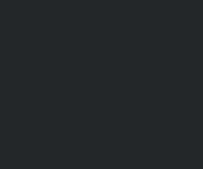
\includegraphics[scale=0.5]{memory/img/1.png}
  \caption{kmalloc/kfree分配逻辑}
\end{figure}


\subsection{虚拟内存设计}

虚拟地址空间其中所有实现全部为基于红黑树的实现。

\subsubsection{\texttt{mm\_struct}}

进程控制块中会维护\texttt{mm\_struct}指针,来管理该进程在虚拟地址空间的信息。\texttt{mm\_struct}结构中主要存储VMA的头,红黑树的根和进程页表的地址。

\begin{lstlisting}[caption=\texttt{mm\_struct}]
struct mm_struct {
  struct vma_struct *root;        // VMA root
  struct vma_struct *mmap_cache;  // Latest used VMA
  struct rb_node mm_rb;           // 红黑树
  int map_count;                  // VMA count
  pgd_t *pgd;                     // Page table entry
  unsigned int start_code, end_code;
  unsigned int start_data, end_data;
  unsigned int start_brk, brk;
  unsigned int start_stack;
};
\end{lstlisting}

\texttt{mm\_struct}指向的红黑树的根可以使得每个进程都有自己可以高效访问的虚拟内存结构。这样可以更好地支持对虚拟内存性能要求较高的一些拓展。

VMA的各项操作都对应红黑树的各项操作。因为没有与文件映射相关的操作,所以把VMA的合并接口留了出来,以后也可以予以拓展。

\begin{lstlisting}[caption=\texttt{vma\_struct}]
struct vma_struct {
  struct mm_struct *vm_mm;
  unsigned long vm_start, vm_end;        // 起止
  struct vma_struct *vm_next;            // 链表结构
  struct vma_struct *vma_left, *vma_right;
  struct rb_node vm_rb;
};

struct vma_struct *find_vma(struct mm_struct *mm, unsigned long addr);
int insert_vm_struct(struct mm_struct *mm, struct vma_struct *vma);
void del_vm_struct(struct vma_struct *vma);
\end{lstlisting}

VMA通过下文自主设计的malloc和free进行申请和释放。在介绍malloc/free之前先简要介绍继承自助教代码结构的TLB。

\subsubsection{TLB}

TLB设计继承自助教组代码,在这里简单提及。

TLB的设计是为了减少虚拟内存到物理内存的转换。而TLB\_refill则是在页表中无法查询到合法虚拟地址值时所作的操作。

遗憾的是此部分是无法体现VMA红黑树结构的正确性的,只能体现虚拟内存的访问,所以另外设计了malloc和free来申请和释放内存从而进行测试。

\subsubsection{malloc/free}

\begin{lstlisting}[caption=malloc/free接口]
int *malloc(unsigned int size);
void free(unsigned int addr);

unsigned long do_map(unsigned long addr, unsigned long len, unsigned long flags);
int do_unmap(unsigned long addr, unsigned long len);
int is_in_vma(unsigned long addr);
\end{lstlisting}

malloc
使用\texttt{get\_unmapped\_area}通过链表循序访问
找到下一个没有被map,同时又大小足够的内存
将这块内存初始化为了VMA
加入当前进程\texttt{mm\_struct}中的红黑树中。

free
将这块VMA取出
检查前后是否为被占用的空间
若未被占用,则合并到空闲链表中
删除其在红黑树中的节点。


\subsubsection{malloc/free导致的内存泄漏}

广义的内存泄漏会在free多个间隔的小内存时发生。尚未对这些泄漏的内存进行整合。从设计角度来说,当内存不够时,可以整合这些小片段,从而提供更多的内存。

\subsubsection{红黑树结构}

红黑树结构与Linux相近,但是删除了Linux中出于vma要映射文件而加入的部分。并重构手写得到。

红黑树关键定义以及部分宏如下。其性质不再赘述。

\begin{lstlisting}[caption=\texttt{struct st\_rb\_node}]
typedef struct st_rb_node {

unsigned long parent_color;
#define RB_RED   1
#define RB_BLACK 0
  struct st_rb_node *left, *right;
}__attribute__((aligned(sizeof(long)))) rb_node;
//对齐是为了把红黑树的颜色挤进节点中,节约空间

#define rb_parent(r)    ((rb_node *)((r)->parent_color & ~3))
#define rb_color(r)     ((r)->parent_color & 1)
#define rb_is_red(r)    (!rb_color(r))
#define rb_is_black(r)  rb_color(r)
#define rb_set_red(r)   do { (r)->parent_color &= ~1; } while (0)
#define rb_set_black(r) do { (r)->parent_color |= 1; } while (0)
\end{lstlisting}


\subsection{总结}

此内存系统在助教组代码的基础上,重构了slab,加入了虚拟内存的红黑树管理,以及设计了malloc和free函数。达到了实现原有设计,同时加以创新的要求。也将VMA合并等接口留好,具有向用户程序加载、页置换等方面的可拓展性。

